\section{Hardware Accelerators}

\begin{figure}[ht]
	\begin{center}
		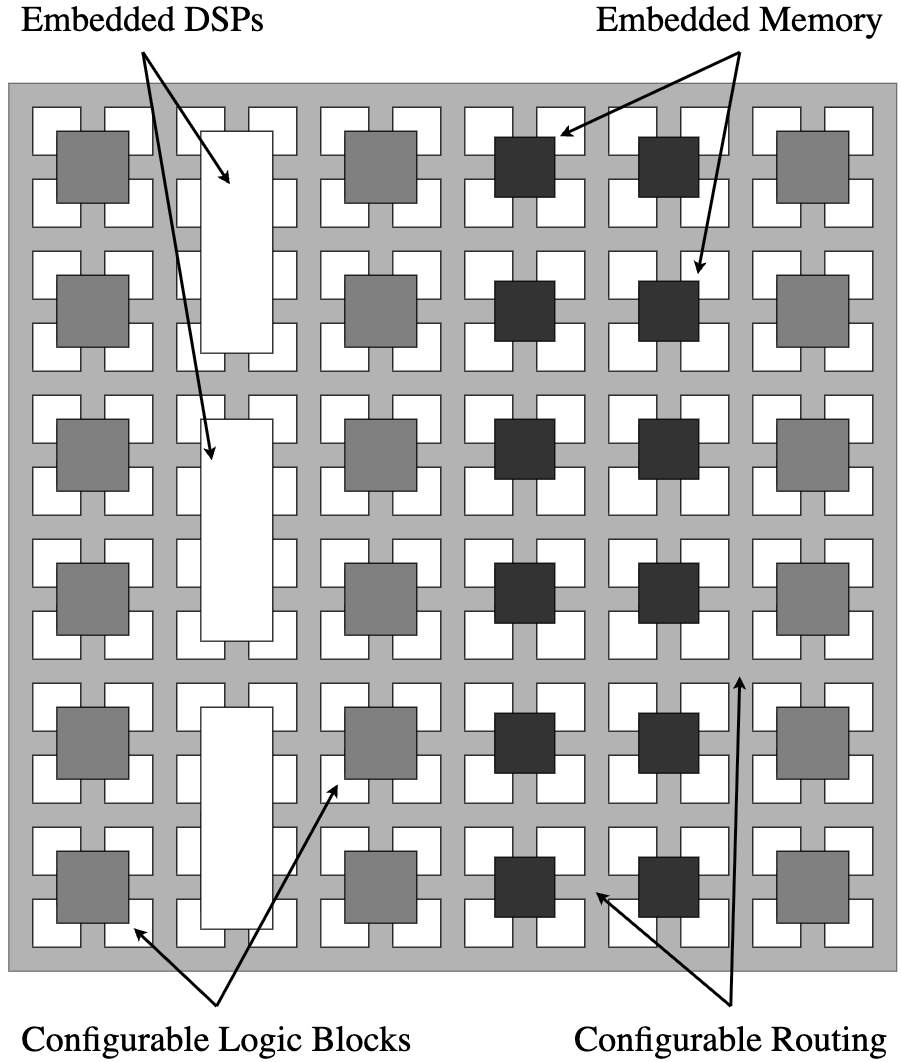
\includegraphics[width=0.55\textwidth]{figures/fpga.png}
	\end{center}
	\caption{General layout of an \acrshort{FPGA}. \acrshort{CLB}s, \acrshort{DSP}s, and memory blocks are placed in a configurable routing network. Figure recreated from \cite{lamoureuxOverviewLowPowerTechniques2008a}.}
	\label{fig:fpga}
\end{figure}

The following section is based on the previous work in \fullcite{noersett2025}.

Designers of embedded real-time systems must balance strict budgets on power, area and cost. Coordinating a large number of simultaneous tasks also presents a significant challenge, and missing deadlines can impact correct functioning and performance of the system. Multiprocessors is an effective approach to designing responsive and robust embedded systems \cite{WOLF2023453}, in which multiple \acrlong{PE}s (\acrshort{PE}) perform tasks in parallel. Parallel execution using a set of simple units can provide the same performance as a single complex unit but at lower cost and power \cite{WOLF2023453, sarpeshkarUniversalPrinciplesUltra2012}.

\acrlong{CPU}s (\acrshort{CPU}), and other programmable \acrshort{PE}s, provide great flexibility. When specialized tasks are to be performed, great improvements in performance can be achieved by use of dedicated hardware accelerators \cite{WOLF2023453}. The \acrfull{GPU} is used in all modern personal computers, and is a great example of the benefits of hardware accelerators. For optimal performance, custom accelerators should be developed and produced as \acrlong{ASIC}s (\acrshort{ASIC}). However, such custom chips are very costly to produce and are only viable for mass produced products. \acrlong{FPGA}s (\acrshort{FPGA}) provide reconfigurable logic, allowing designers to implement custom logic at a fraction of the price. Typically, \acrshort{FPGA}s can be reprogrammed, providing great flexibility for remotely deployed systems.

A typical layout of an \acrshort{FPGA} is shown in \autoref{fig:fpga}. A configurable routing network connects an array of components. \acrlong{CLB}s (\acrshort{CLB}) can be programmed to provide any logic function. This is achieved by use of \acrlong{LUT}s (\acrshort{LUT}) and \acrlong{FF}s (\acrshort{FF}). Additional, specialized components serve to improve the area footprint, power and computational performance of the chip. \acrfull{BRAM} provides data storage, whereas \acrlong{DSP}s (\acrshort{DSP}) provide arithmetic functions such as addition, multiplication and bit manipulation. The hardware resource utilization of a custom logic design is measured in the amount of \acrshort{LUT}s, \acrshort{FF}s, \acrshort{DSP}s and \acrshort{BRAM} that is occupied by the design.

Pipelining is a technique employed by digital processors, and accelerators, to provide computational parallelism within a single processing core. Independent operations are split by pipeline registers, dubbed pipeline stages, allowing a high clock frequency. At each clock edge, new data is input to the pipeline, allowing parallel computation across the pipeline stages. The clock frequency is limited by the longest electrical path between the pipeline registers of any pipeline stage. Static timing analysis can provide estimates of the path that limits the frequency (critical path), and thus the achievable speed of the circuit.

Design of custom logic presents additional challenges in terms of design complexity and development time as compared to software. Designs are typically conceptualised at a microarchitectural level, using block diagrams, before conversion to \acrfull{RTL}. \acrshort{RTL} is represented using languages such as VHDL, Verilog or Systemverilog and describes how data moves between registers and which operations are performed on the data in-between them. \acrshort{RTL} code is converted, synthesized, to a gatelevel netlist, in which the design is represented using pure logic gates (AND, OR, NAND, \dots). Through a process named \acrfull{PnR}, the gatelevel netlist is mapped to a physical layout for \acrshort{ASIC}, or to the components of an \acrshort{FPGA}.

\acrfull{HLS} provides an alternative design flow which attempts to alleviate the long design time of \acrshort{RTL} code. The algorithm that is to be implemented is first described in a high-level language such as C or C++. This high-level description is then converted to \acrshort{RTL} by automated tools \cite{barriosHardwareImplementationCCSDS2021}. However, these tools produce suboptimal results compared to manually describing the design in the \acrshort{RTL} abstraction. Skilled design engineers can optimize the code for higher frequencies, lower power and area footprint.

Before the accelerator design is deployed to real hardware, extensive testing must be performed to verify the correct, logical functioning of the design. Verification can be performed at all stages of the design flow: at the RTL level, gate level and the final technology mapped design. The main part of verification is typically done using simulation at the \acrshort{RTL} level. A typical test structure applies test data to the \acrfull{DUT} and probes internal signals. The outputs, and intermediate values, are then compared to a reference model, dubbed a golden model, written in a high-level language. The most challenging part is to produce a set of test data that ensures sufficient coverage of the corner cases of the design. Extensive testing, checking all possible values, is for non-trivial designs not a viable approach. Two main approaches are used to ensure functional correctness: constrained random verification and coverage data. Constrained random verification combines randomly generated test data with special test sets that target known corner cases. Data is also constrained within the confines of possible values. Collected coverage data tracks whether identified corner cases are tested by the randomly generated data.

The power consumption of logic designs is measured in terms of static and dynamic power \cite{sarpeshkarUniversalPrinciplesUltra2012}. Static power consumption is the power consumed by the circuit in its idle state, that is when the clock signals are turned off and internal values do not change. This is due to leakage currents in the transistors, an effect which is magnified as transistor sizes are reduced. Dynamic power is caused by the switching of transistor states. As a transistor switches between its on and off states, current is leaked. Dynamic power increases with the clock frequency, as transistor states switch more frequently. Both the static and dynamic power increases as the number of gates in a circuit increases.

To reduce the cost of developing cube satellites, such as the \acrshort{hypso} mission, commercially available \acrfull{COTS} are used. As an example, the processing system on-board the \acrshort{hypso}-1 and 2 use an \acrshort{MPSoC} from AMD (formerly Xilinx) named the Zynq-7030. The chip embeds two ARM processing units, an embedded \acrshort{GPU}, and a wide range of hardware peripherals that support common communication protocols, as well as \acrlong{ADC}s (\acrshort{ADC}), timers and other useful features. Additionally, the chip includes an embedded \acrshort{FPGA} which has direct access to the internal system data bus. This means that custom logic designs can interface with the \acrshort{CPU}s and other peripherals using common data bus interfaces such as \acrshort{AXI}, developed by ARM. The internal data bus can connect to external \acrshort{RAM}, which means that data can be moved to and from the custom logic using \acrfull{DMA} without intervention from the \acrshort{CPU}s. Embedding custom and fixed hardware in the same chip also reduces the physical spacing between components, further increasing processing speed and power efficiency.
